\documentclass[12pt,letterpaper]{article}
\usepackage{fullpage}
\usepackage[top=2cm, bottom=4.5cm, left=2.5cm, right=2.5cm]{geometry}
\usepackage{amsmath,amsthm,amsfonts,amssymb,amscd}
\usepackage{lastpage}
\usepackage{enumerate}
\usepackage{fancyhdr}
\usepackage{mathrsfs}
\usepackage{xcolor}
\usepackage{graphicx}
\usepackage{listings}
\usepackage{hyperref}

\hypersetup{%
  colorlinks=true,
  linkcolor=blue,
  linkbordercolor={0 0 1}
}
 
\renewcommand\lstlistingname{Algorithm}
\renewcommand\lstlistlistingname{Algorithms}
\def\lstlistingautorefname{Alg.}

\lstdefinestyle{Python}{
    language        = Python,
    frame           = lines, 
    basicstyle      = \footnotesize,
    keywordstyle    = \color{blue},
    stringstyle     = \color{green},
    commentstyle    = \color{red}\ttfamily
}

\setlength{\parindent}{0.0in}
\setlength{\parskip}{0.05in}

% Edit these as appropriate
\newcommand\course{APL 452}
\newcommand\hwnumber{1}                  % <-- homework number
\newcommand\NetIDa{2019ME10770}           % <-- NetID of person #1
\newcommand\NetIDb{Aditya Shankar Garg}           % <-- NetID of person #2 (Comment this line out for problem sets)

\pagestyle{fancyplain}
\headheight 35pt
\lhead{\NetIDa}
\lhead{\NetIDa\\\NetIDb}                 % <-- Comment this line out for problem sets (make sure you are person #1)
\chead{\textbf{\Large Homework \hwnumber}}
\rhead{\course \\ \today}
\lfoot{}
\cfoot{}
\rfoot{\small\thepage}
\headsep 1.5em

\begin{document}

\section*{Problem 5}

\textbf{derive the v-stage runge-kutta method that corresponds to the given collocation points}
\newline
\newline
we have the following relations : 
\[ a_{ji} = \int_{0}^{c_j} l_i(\tau)d\tau\]
\[b_j = \int_{0}^{1} l_i(\tau)d\tau \]

we also know that the form of $l_i(\tau)$ can be given by the following expression : 

\[l_i(\tau) = \prod_{k = 1, k \not= i}^{3} \frac{\tau - c_k}{c_i - c_k}\]

we need to evaluate the integrals ; let us start with $i=1, j=1$  and try to compute $a_{11}$ as follows:

\[ a_{11} = \int_{0}^{\frac{1}{4}} \frac{\tau-\frac{1}{2}}{\frac{1}{4} - \frac{1}{2}} \cdot  \frac{\tau-\frac{3}{4}}{\frac{1}{4} - \frac{3}{4}}d\tau = 8 \cdot \int_{0}^{\frac{1}{4}} \left(\tau-\frac{1}{2}\right) \cdot  \left(\tau-\frac{3}{4}\right) d\tau = 8 \cdot \frac{23}{384} = \frac{23}{48} \]

\[ a_{12} = \int_{0}^{\frac{1}{4}} \frac{\tau-\frac{1}{4}}{\frac{1}{2} - \frac{1}{4}} \cdot  \frac{\tau-\frac{3}{4}}{\frac{1}{2} - \frac{3}{4}}d\tau = -16 \cdot \int_{0}^{\frac{1}{4}} \left(\tau-\frac{1}{4}\right) \cdot  \left(\tau-\frac{3}{4}\right) d\tau = -16 \cdot \frac{1}{48} = -\frac{1}{3} \]

\[ a_{13} = \int_{0}^{\frac{1}{4}} \frac{\tau-\frac{1}{4}}{\frac{3}{4} - \frac{1}{4}} \cdot  \frac{\tau-\frac{1}{2}}{\frac{3}{4} - \frac{1}{2}}d\tau = 8 \cdot \int_{0}^{\frac{1}{4}} \left(\tau-\frac{1}{4}\right) \cdot  \left(\tau-\frac{1}{2}\right) d\tau = 8 \cdot \frac{5}{384} = \frac{5}{48} \]

\[ a_{21} = \int_{0}^{\frac{1}{2}} \frac{\tau-\frac{1}{2}}{\frac{1}{4} - \frac{1}{2}} \cdot  \frac{\tau-\frac{3}{4}}{\frac{1}{4} - \frac{3}{4}}d\tau = 8 \cdot \int_{0}^{\frac{1}{2}} \left(\tau-\frac{1}{2}\right) \cdot  \left(\tau-\frac{3}{4}\right) d\tau = 8 \cdot \frac{7}{96} = \frac{7}{12} \]

\[ a_{22} = \int_{0}^{\frac{1}{2}} \frac{\tau-\frac{1}{4}}{\frac{1}{2} - \frac{1}{4}} \cdot  \frac{\tau-\frac{3}{4}}{\frac{1}{2} - \frac{3}{4}}d\tau = -16 \cdot \int_{0}^{\frac{1}{2}} \left(\tau-\frac{1}{4}\right) \cdot  \left(\tau-\frac{3}{4}\right) d\tau = -16 \cdot \frac{1}{96} = -\frac{1}{6} \]

\[ a_{23} = \int_{0}^{\frac{1}{2}} \frac{\tau-\frac{1}{4}}{\frac{3}{4} - \frac{1}{4}} \cdot  \frac{\tau-\frac{1}{2}}{\frac{3}{4} - \frac{1}{2}}d\tau = 8 \cdot \int_{0}^{\frac{1}{2}} \left(\tau-\frac{1}{4}\right) \cdot  \left(\tau-\frac{1}{2}\right) d\tau = 8 \cdot \frac{1}{96} = \frac{1}{12} \]

we can similarly compute $a_{31}, a_{32}, a_{33}$ and that will come out to be : $\frac{9}{16}, 0, \frac{7}{16}$ respectively and then we should compute $b_j$'s as follows :

\[b_1 =  8 \int_{0}^{1} \left(\tau - \frac{1}{2}\right) \cdot \left(\tau - \frac{3}{4}\right) d\tau = \frac{2}{3}\]
\[b_2 =  -16 \int_{0}^{1} \left(\tau - \frac{1}{4}\right) \cdot \left(\tau - \frac{3}{4}\right) d\tau = -\frac{1}{3}\]
\[b_3 =  8 \int_{0}^{1} \left(\tau - \frac{1}{4}\right) \cdot \left(\tau - \frac{1}{2}\right) d\tau = \frac{2}{3}\]

hence we have a butcher tableau for the runge-kutta with the given collocation points as shown in the figure below : 

\begin{center}
    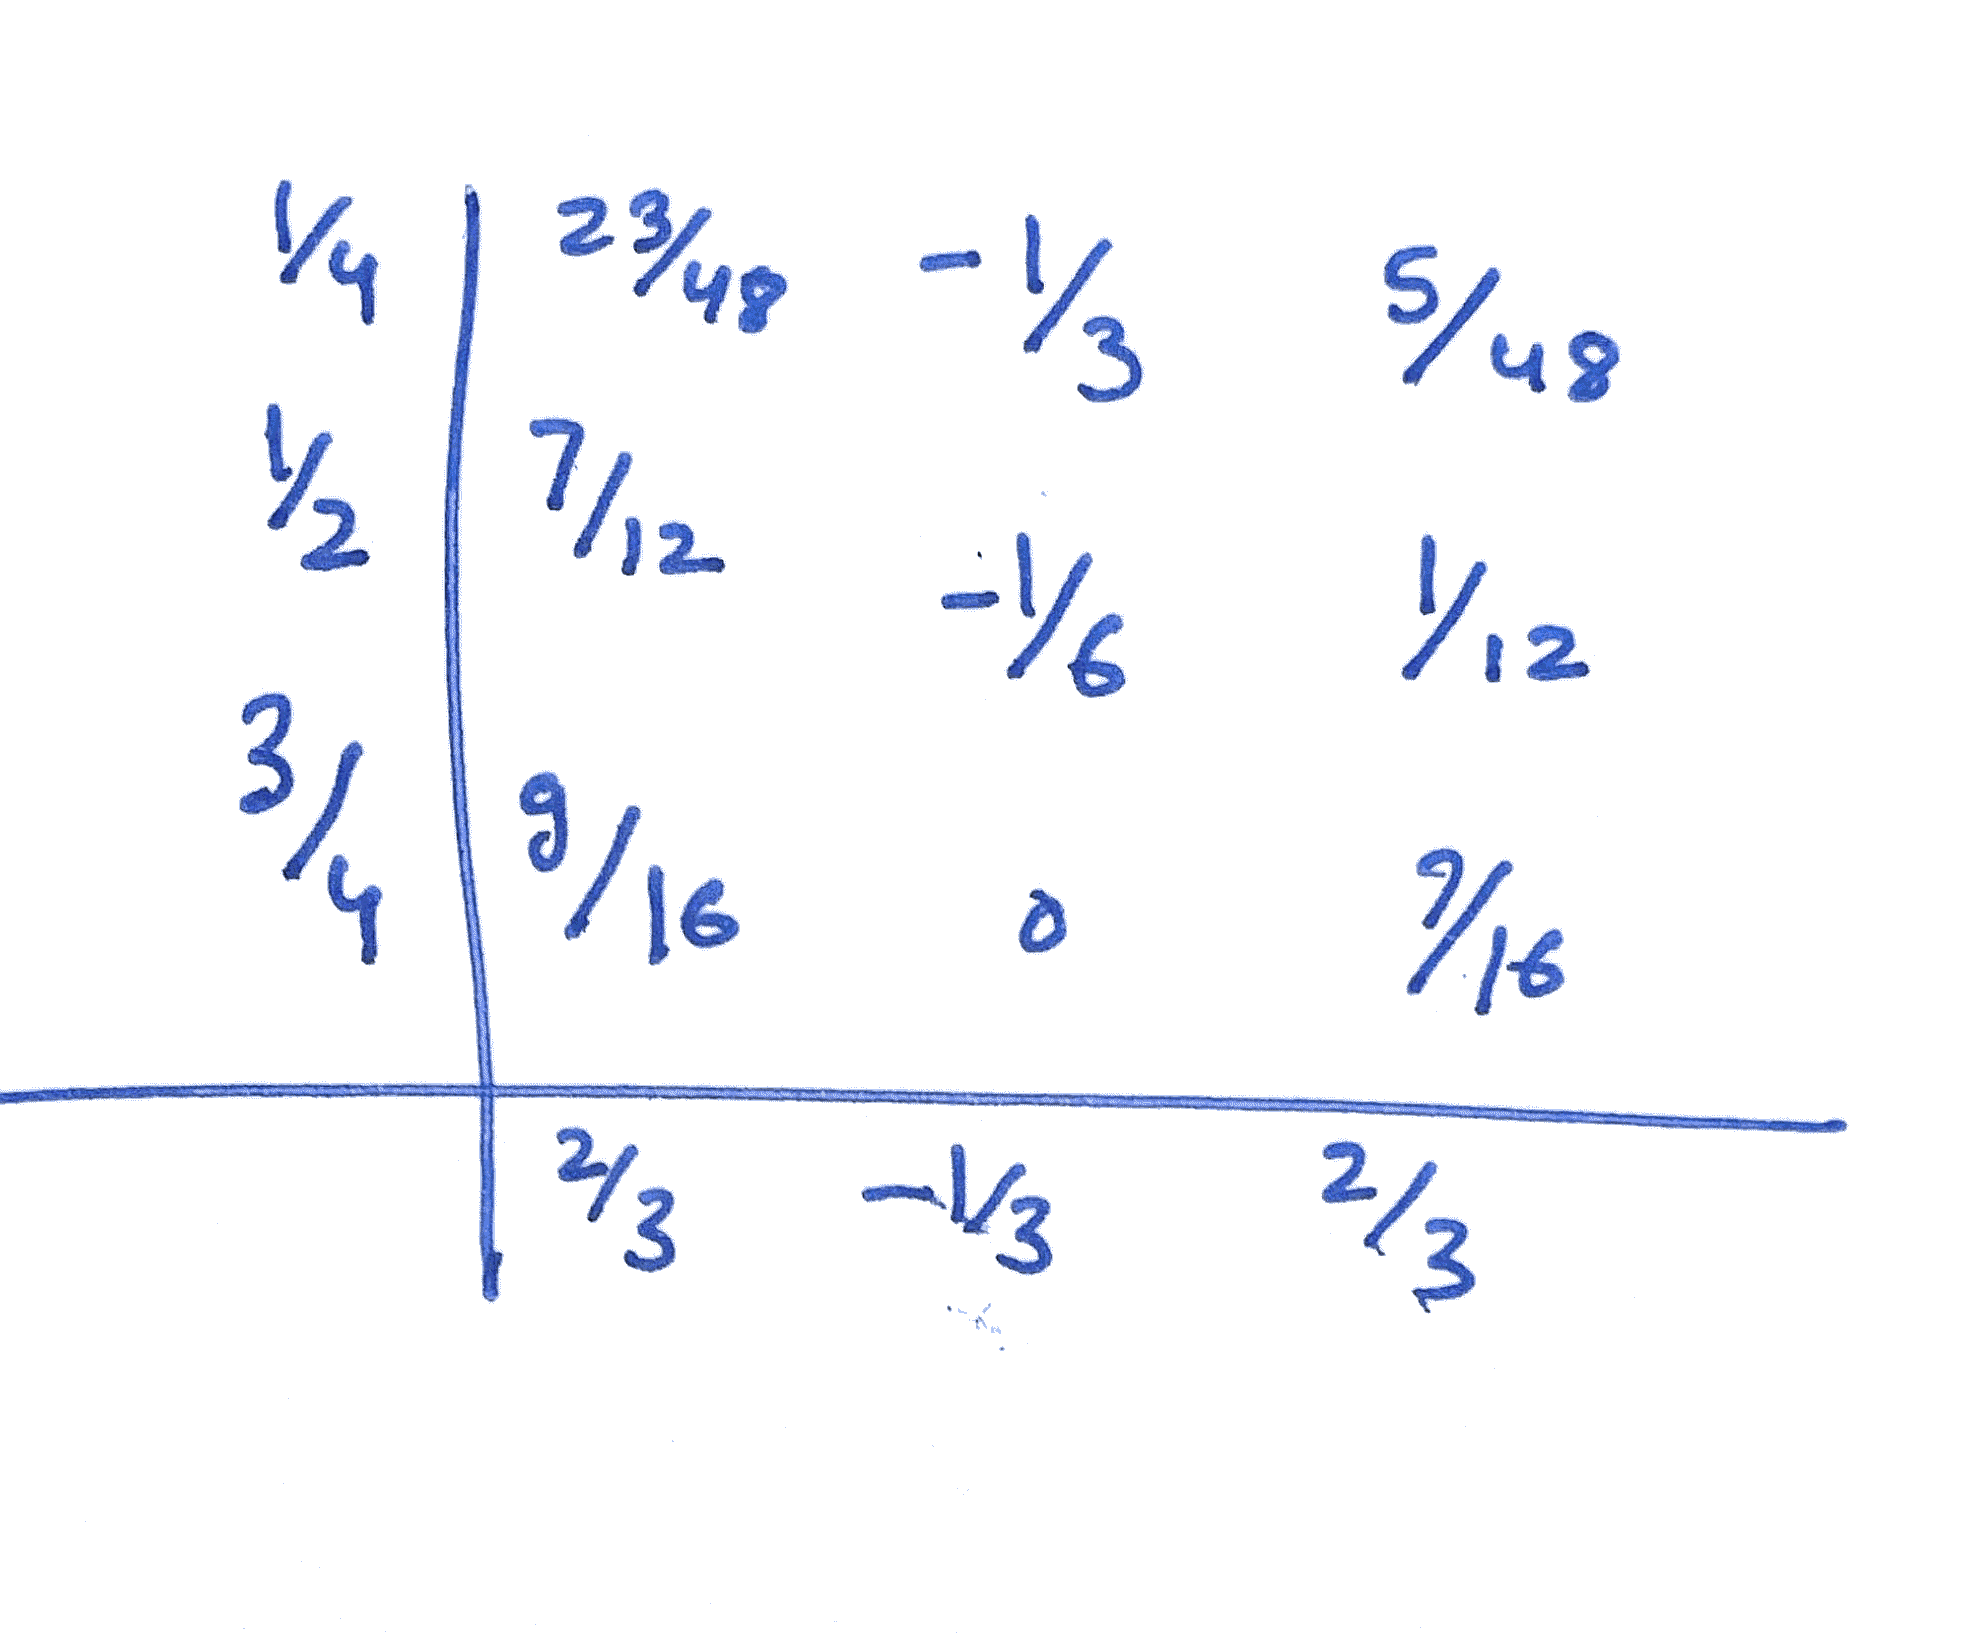
\includegraphics[scale=0.1]{file_2.png}
\end{center}
\newline
we can also find the order for the method using the root polynomial defined by :  $g(\tau) = \left(\tau - \frac{1}{4}\right) \left(\tau - \frac{1}{2}\right) \left(\tau - \frac{3}{4}\right)$ 
\newline
\newline
we need to check for what least value of $m$ does the integral given by :
\[I_m = \int_{0}^{1} t^m g(\tau) d\tau \not= 0\]

this relation is satisfied for $m=1$ and so the order is given by $v + m = 3 + 1 = 4$
\end{document}